
%\documentstyle[epsf,twocolumn]{jarticle}       %LaTeX2e仕様
% \documentclass[twocolumn]{jarticle}     %pLaTeX2e仕様(platex.exeの場合)
\documentclass[onecolumn]{ujarticle}   %pLaTeX2e仕様(uplatex.exeの場合)
%%%%%%%%%%%%%%%%%%%%%%%%%%%%%%%%%%%%%%%%%%%%%%%%%%%%%%%%%%%%%%
%%
%%  基本バージョン
%%
%%%%%%%%%%%%%%%%%%%%%%%%%%%%%%%%%%%%%%%%%%%%%%%%%%%%%%%%%%%%%%%%
\setlength{\topmargin}{-45pt}
%\setlength{\oddsidemargin}{0cm}
\setlength{\oddsidemargin}{-7.5mm}
%\setlength{\evensidemargin}{0cm}
\setlength{\textheight}{24.1cm}
%setlength{\textheight}{25cm}
\setlength{\textwidth}{17.4cm}
%\setlength{\textwidth}{172mm}
\setlength{\columnsep}{11mm}

%\kanjiskip=.07zw plus.5pt minus.5pt


% 【節が変わるごとに (1.1)(1.2) … (2.1)(2.2) と数式番号をつけるとき】
%\makeatletter
%\renewcommand{\theequation}{%
%\thesection.\arabic{equation}} %\@addtoreset{equation}{section}
%\makeatother

%\renewcommand{\arraystretch}{0.95} 行間の設定
%%%%%%%%%%%%%%%%%%%%%%%%%%%%%%%%%%%%%%%%%%%%%%%%%%%%%%%%
%\usepackage{graphicx}   %pLaTeX2e仕様(\documentstyle ->\documentclass)
\usepackage[dvipdfmx]{graphicx}
\usepackage{subcaption}
\usepackage{multirow}
\usepackage{amsmath}
\usepackage{url}
\usepackage{ulem}
\usepackage{algorithm}
\usepackage{algorithmic}
\usepackage{listings} %,jlisting} %日本語のコメントアウトをする場合jlistingが必要
%ここからソースコードの表示に関する設定
\lstset{
  basicstyle={\ttfamily},
  identifierstyle={\small},
  commentstyle={\smallitshape},
  keywordstyle={\small\bfseries},
  ndkeywordstyle={\small},
  stringstyle={\small\ttfamily},
  frame={tb},
  breaklines=true,
  columns=[l]{fullflexible},
  numbers=left,
  xrightmargin=0zw,
  xleftmargin=3zw,
  numberstyle={\scriptsize},
  stepnumber=1,
  numbersep=1zw,
  lineskip=-0.5ex
}
\newcommand{\argmax}{\mathop{\rm arg~max}\limits}
\newcommand{\argmin}{\mathop{\rm arg~min}\limits}

%%%%%%%%%%%%%%%%%%%%%%%%%%%%%%%%%%%%%%%%%%%%%%%%%%%%%%%%
\begin{document}

	%bibtex用の設定
	%\bibliographystyle{ujarticle}

	% \twocolumn[
		\noindent
		\hspace{1em}
		2022 年 6 月 24 日
		ゼミ資料
		\hfill
		杉山 竜弥
		\vspace{2mm}

		\hrule
		\begin{center}
			{\Large \bf 進捗報告}
		\end{center}
		\hrule
		\vspace{9mm}
	% ]


\section{今週やったこと}
\begin{itemize}
  \item スケッチ分割
\end{itemize}


\section{スケッチ分割}
% score/index= 0.03659976387249114 135
% [1]
% score/index= 0.020360219263899765 331
% [2]
% score/index= 0.017004936917169502 49
% [3]
% score/index= 0.015701898289196155 49
% [4]
% score/index= 0.011605700014690759 49
% [5]
% score/index= 0.011412072047298227 119
% [6]
% score/index= 0.01093591047812818 119
% result :  0.03659976387249114 135 0
% akaze= 27.322580645161292
% sim label= hamburger
% Out[2]: (0.03659976387249114, 135)

% comparing [sheep]
% [0]
% score/index= 0.013263525305410123 61 #car
% [1]
% score/index= 0.011115138335145583 149 #hot air balloon
% [2]
% score/index= 0.01107999512967247 149
% [3]
% score/index= 0.01107999512967247 149
% [4]
% score/index= 0.010104166666666666 149
% [5]
% score/index= 0.009319950839819745 48 #bush
% result :  0.013263525305410123 61 0
% akaze= 75.39473684210526
% sim label= car
% Out[3]: (0.013263525305410123, 61)
% \begin{figure}[th]
%   \begin{center}
%     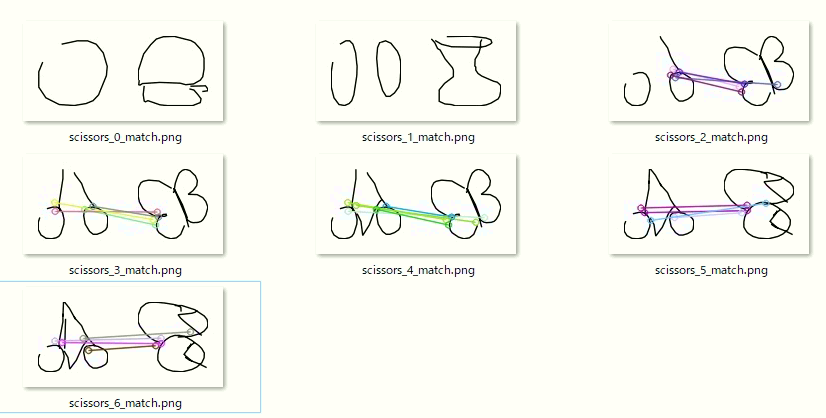
\includegraphics[clip,width=100mm]{scissors.png}
%     \caption{「ハサミ」クラスと類似したスケッチ}
%     \label{fig:result1_1}
%   \end{center}
% \end{figure}

% comparing [sun]
% [0]
% score/index= 0.03873873873873874 73 clock
% [1]
% score/index= 0.023554603854389723 272
% [2]
% score/index= 0.019246190858059342 272
% [3]
% score/index= 0.016277641277641277 339 wine bottle
% [4]
% score/index= 0.015432980851671907 272
% [5]
% score/index= 0.013841670713938804 272 snowmax
% result :  0.03873873873873874 73 0
% akaze= 25.813953488372093
% sim label= clock
% Out[4]: (0.03873873873873874, 73)

スケッチを分割し,quick draw データセットから抜粋した345 クラスについて,
もっとも類似しているクラスを検索した.
分割方法は 1 筆ごとの過程とし,
類似度は AKAZE とした.

「ヒツジ」クラスは,車,気球,低木と類似し,最も AKAZE 類似度が高かったのは,
1 筆目のみの場合で 25.8 となった.
主観ではヒツジと低木が似ていると思われたが,
異常に低い値の車が選ばれた.

「太陽」クラスでは,時計,雪だるま,ワインボトルが各々の部分スケッチで選ばれ,
最終的に同じく 1 筆目の場合の,時計が最も高い類似度となった.
主観では比較的妥当であるが,「円」が選ばれなかったことが気になる.

スケッチの分割を AKAZE で試した結果について,
ある程度妥当だが,間に合わなかった他の類似度も試したい.
また 1 筆目が選ばれる場合が多かったが,
書き込んでいくと対象のクラスに近づくので当然の結果と言える.
分割方法を全通りににするなどで,改良したい.

\begin{figure}[th]
  \begin{center}
    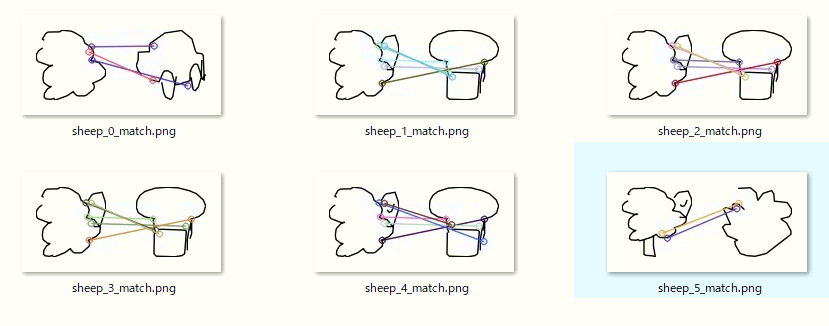
\includegraphics[clip,width=140mm]{sheep.png}
    \caption{「ヒツジ」クラスと類似したスケッチ}
    \label{fig:result1_2}
  \end{center}
\end{figure}

\begin{figure}[htbp]
    \begin{tabular}{cc}
      \begin{minipage}[t]{0.45\hsize}
        \centering
        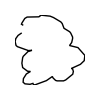
\includegraphics[keepaspectratio, scale=1]{sheep_0_best.png}
        \caption{最尤部分スケッチ}
        \label{fig:result2_1}
      \end{minipage} &
      \begin{minipage}[t]{0.45\hsize}
        \centering
        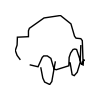
\includegraphics[keepaspectratio, scale=1]{sheep_car_sim.png}
        \caption{類似スケッチ(車)}
        \label{fig:result2_2}
      \end{minipage} \\

    \end{tabular}
  \end{figure}


  \begin{figure}[th]
    \begin{center}
      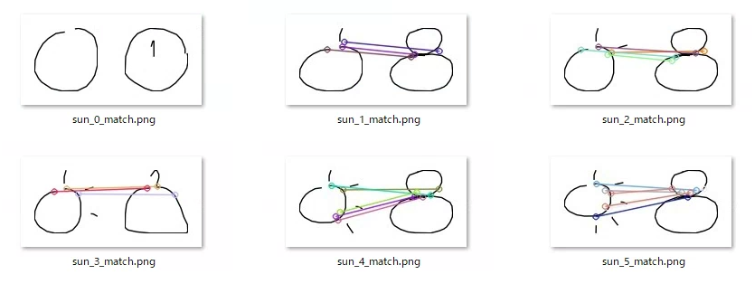
\includegraphics[clip,width=140mm]{sun.png}
      \caption{「太陽」クラスと類似したスケッチ}
      \label{fig:result1_2}
    \end{center}
  \end{figure}

  \begin{figure}[htbp]
      \begin{tabular}{cc}
        \begin{minipage}[t]{0.45\hsize}
          \centering
          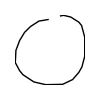
\includegraphics[keepaspectratio, scale=1]{sun_0_best.png}
          \caption{最尤部分スケッチ}
          \label{fig:result2_1}
        \end{minipage} &
        \begin{minipage}[t]{0.45\hsize}
          \centering
          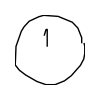
\includegraphics[keepaspectratio, scale=1]{sun_clock_sim.png}
          \caption{類似スケッチ(時計)}
          \label{fig:result2_2}
        \end{minipage} \\

      \end{tabular}
    \end{figure}

\section{予定}
\begin{itemize}
  \item 類似度を描き順にした場合の実験.
  \item 資料作成
\end{itemize}


% \begin{figure}[h]
%   \begin{center}
%     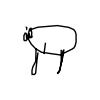
\includegraphics[clip,width=20mm]{decode1.png}
%     \caption{比較元のデコードスケッチ}
%     \label{fig:result2_1}
%   \end{center}
% \end{figure}

% 参考文献リスト
% \bibliographystyle{unsrt}
% \bibliography{ref}
\end{document}
